\documentclass[11pt]{beamer}
\usetheme{Warsaw}
\usepackage[utf8]{inputenc}
\usepackage[french]{babel}
\usepackage[T1]{fontenc}
\usepackage{amsmath}
\usepackage{amsfonts}
\usepackage{amssymb}
\usepackage{graphicx}
\usepackage{caption}
%%\usepackage[utf8x]{inputenc}
\usepackage[T1]{fontenc}
\usepackage{lmodern}

\usepackage{ifthen}
\usepackage{url}


\usepackage{multirow}

% Color
% cfr http://en.wikibooks.org/wiki/LaTeX/Colors
\usepackage{color}
\usepackage[usenames,dvipsnames,svgnames,table]{xcolor}
\definecolor{dkgreen}{rgb}{0.25,0.7,0.35}
\definecolor{dkred}{rgb}{0.7,0,0}

\newcommand{\matlab}{\textsc{Matlab}}

% Math symbols
\usepackage{amsmath}
\usepackage{amssymb}
\usepackage{amsthm}
\DeclareMathOperator*{\argmin}{arg\,min}
\DeclareMathOperator*{\argmax}{arg\,max}


% Sets
\newcommand{\Z}{\mathbb{Z}}
\newcommand{\R}{\mathbb{R}}
\newcommand{\Rn}{\R^n}
\newcommand{\Rnn}{\R^{n \times n}}
\newcommand{\C}{\mathbb{C}}
\newcommand{\K}{\mathbb{K}}
\newcommand{\Kn}{\K^n}
\newcommand{\Knn}{\K^{n \times n}}

% Unit vectors
\usepackage{esint}
\usepackage{esvect}
\newcommand{\kmath}{k}
\newcommand{\xunit}{\hat{\imath}}
\newcommand{\yunit}{\hat{\jmath}}
\newcommand{\zunit}{\hat{\kmath}}
\newcommand{\uunit}{\hat{\umath}}

% rot & div & grad & lap
\DeclareMathOperator{\newdiv}{div}
\newcommand{\divn}[1]{\nabla \cdot #1}
\newcommand{\rotn}[1]{\nabla \times #1}
\newcommand{\grad}[1]{\nabla #1}
\newcommand{\gradn}[1]{\nabla #1}
\newcommand{\lap}[1]{\nabla^2 #1}


% Elec
\newcommand{\B}{\vec B}
\newcommand{\E}{\vec E}
\newcommand{\EMF}{\mathcal{E}}
\newcommand{\perm}{\varepsilon} % permittivity

\newcommand{\bigoh}{\mathcal{O}}
\newcommand\eqdef{\triangleq}

\DeclareMathOperator{\newdiff}{d} % use \dif instead
\newcommand{\dif}{\newdiff\!}
\newcommand{\fpart}[2]{\frac{\partial #1}{\partial #2}}
\newcommand{\ffpart}[2]{\frac{\partial^2 #1}{\partial #2^2}}
\newcommand{\fdpart}[3]{\frac{\partial^2 #1}{\partial #2\partial #3}}
\newcommand{\fdif}[2]{\frac{\dif #1}{\dif #2}}
\newcommand{\ffdif}[2]{\frac{\dif^2 #1}{\dif #2^2}}
\newcommand{\constant}{\ensuremath{\mathrm{cst}}}

\usepackage{siunitx}

\usepackage{tikz}

\usepackage{pgfplots}
\usepackage{lmodern}
\usepackage{microtype}
\usepackage{xspace}

\usepackage{babel}
% Listing
% always put it after babel
% http://tex.stackexchange.com/questions/100717/code-in-lstlisting-breaks-document-compile-error
\usepackage{listings}

\definecolor{mygreen}{rgb}{0,0.6,0}
\definecolor{mygray}{rgb}{0.5,0.5,0.5}
\definecolor{mymauve}{rgb}{0.58,0,0.82}
\lstset{ %
  language=Matlab,
  backgroundcolor=\color{white},   % choose the background color; you must add \usepackage{color} or \usepackage{xcolor}
  basicstyle=\footnotesize,        % the size of the fonts that are used for the code
  breakatwhitespace=false,         % sets if automatic breaks should only happen at whitespace
  breaklines=true,                 % sets automatic line breaking
  captionpos=b,                    % sets the caption-position to bottom
  commentstyle=\color{mygreen},    % comment style
  deletekeywords={...},            % if you want to delete keywords from the given language
  escapeinside={\%*}{*)},          % if you want to add LaTeX within your code
  extendedchars=true,              % lets you use non-ASCII characters; for 8-bits encodings only, does not work with UTF-8
  frame=single,	                   % adds a frame around the code
  keepspaces=true,                 % keeps spaces in text, useful for keeping indentation of code (possibly needs columns=flexible)
  keywordstyle=\color{blue},       % keyword style
  otherkeywords={*,...},           % if you want to add more keywords to the set
  numbers=none,                    % where to put the line-numbers; possible values are (none, left, right)
  numbersep=5pt,                   % how far the line-numbers are from the code
  numberstyle=\tiny\color{mygray}, % the style that is used for the line-numbers
  rulecolor=\color{black},         % if not set, the frame-color may be changed on line-breaks within not-black text (e.g. comments (green here))
  showspaces=false,                % show spaces everywhere adding particular underscores; it overrides 'showstringspaces'
  showstringspaces=false,          % underline spaces within strings only
  showtabs=false,                  % show tabs within strings adding particular underscores
  stepnumber=2,                    % the step between two line-numbers. If it's 1, each line will be numbered
  stringstyle=\color{mymauve},     % string literal style
  tabsize=2,	                   % sets default tabsize to 2 spaces
  title=\lstname                   % show the filename of files included with \lstinputlisting; also try caption instead of title
}

\KOMAoptions{DIV=last}

\usepackage[top = 2.5 cm, bottom = 3 cm, left = 2.5 cm, right = 2.5 cm]{geometry}
\usepackage{caption}

\title{LELEC2103 - Projet 3 in Electricity}
\subtitle[\ldots]{Result of the lab 5 and lab 6}
\author[D. Deprez\and B. Ouachalih]{Damien Deprez\and Bilal Ouachalih}
\institute{EPL}
\date{16th december 2016}

\begin{document}

% TITLE PAGE
{
	\setbeamertemplate{headline}{}  
	\setbeamertemplate{footline}{}
	\setbeamertemplate{navigation symbols}{}
	\begin{frame}[noframenumbering]
		\titlepage
	\end{frame}
} 

% TABLE OF CONTENTS
{
	\setbeamertemplate{navigation symbols}{}
	\setbeamertemplate{headline}{}
	\begin{frame}[noframenumbering]{Plan de la présentation}
		\tableofcontents
	\end{frame}
}

\section{Frame detection and frequency offset correction}

\subsection{Frame detection}

\begin{frame}
\frametitle{Frame detection}
\begin{itemize}
\item The received signal is
\begin{equation}
y[n] = hs[n-d] + v[n]
\end{equation}
with $h$ the channel coefficient and $d$ the frame offset.
\item The correlation with the training sequence is given by
\begin{equation}
R[n] = \left| \sum_{k=0}^{N_t-1} t^*[k]y[n+k] \right|^2
\end{equation}
with $\{t[n]\}_0^{N_t-1}$ is the known training sequence. \\
In the lab, it's 4 ength 11 Barker Sequence
\item With the good correlation properties of the training sequence, the frame offset is given by 
\begin{equation}
\hat{d} = argmax_n{R[n]}
\end{equation}
\end{itemize}

\end{frame}


\subsection{Frequency offset estimation}
\begin{frame}
\frametitle{Frequency offset estimation}
\begin{itemize}
\item The received signal is
\begin{equation}
y[n] = e^{j2\pi \epsilon n} \sum_{l=0}^{L}{h[l]s[n-l]+v[n]}
\end{equation}
with $\epsilon = f_0 T$ the offset.
\item To estimate the offset, we use the Moose method.
\begin{equation}
\hat{\epsilon} = \frac{\text{phase} \sum_{l=L}^{N_t-1}{y[l+N_t]y^*[l]}}{2\pi N_t}
\end{equation}

\end{itemize}

\end{frame}

\subsection{Limit of the method}

\begin{frame}
\frametitle{Maximum frequency offset}
\begin{minipage}[b]{0.48\linewidth}
        \centering 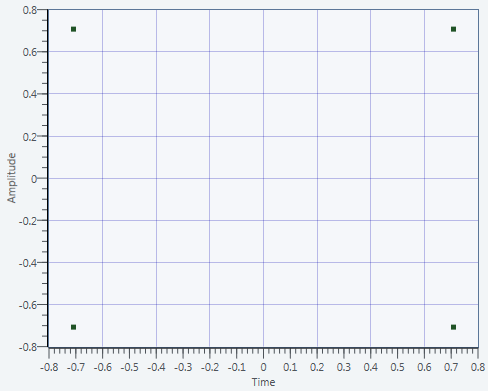
\includegraphics[scale=0.35]{img/Moose_Limit_10k.png}
     \captionof{figure}{\label{fig:Moose_10k}Frequency offset of 10kHz}
    \end{minipage}\hfill
    \begin{minipage}[b]{0.48\linewidth}
         \centering 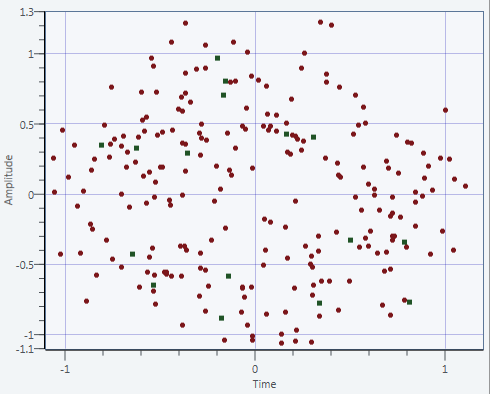
\includegraphics[scale=0.35]{img/Moose_Limit_12k.png}
         \captionof{figure}{\label{fig:Moose_12k}Frequency offset of 12kHz}
    \end{minipage}
\begin{itemize}
\item The Moose method has a limit 
\begin{equation}
|\epsilon| \leq \frac{1}{2N_t}
\end{equation}
\end{itemize}
\end{frame}

\subsection{Result}
\subsubsection{Constellation}

\begin{frame}
\frametitle{Result - Constellation}
\begin{minipage}[b]{0.48\linewidth}
        \centering 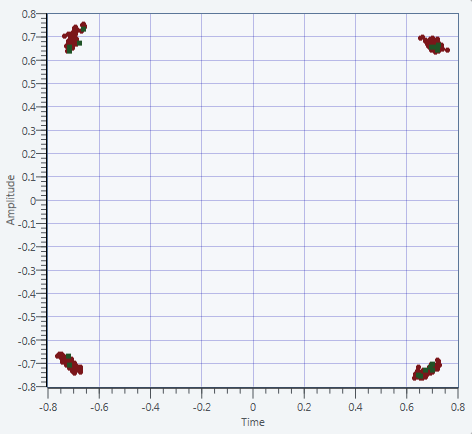
\includegraphics[scale=0.35]{img/USRP_carrieroffset_227.png}
     \captionof{figure}{\label{fig:USRP_227}USRP with Frequency offset of 227 Hz}
    \end{minipage}\hfill
    \begin{minipage}[b]{0.48\linewidth}
         \centering 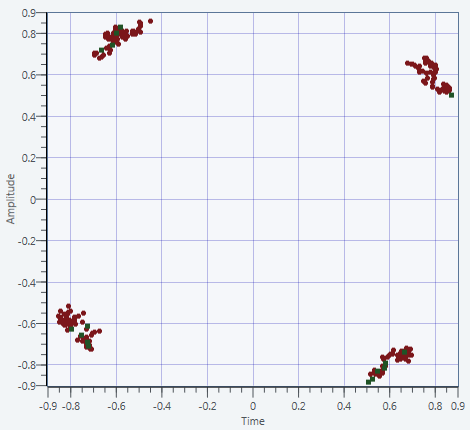
\includegraphics[scale=0.35]{img/USRP_carrieroffset_1818}
         \captionof{figure}{\label{fig:Moose_1818}USRP with Frequency offset of 1818 Hz}
    \end{minipage}

\end{frame}

% TABLE OF CONTENTS
{
	\setbeamertemplate{navigation symbols}{}
	\setbeamertemplate{headline}{}
	\begin{frame}[noframenumbering]{Plan de la présentation}
		\tableofcontents
	\end{frame}
}

\section{OFDM modulation}
\begin{frame}
\frametitle{Modulation}

\begin{figure}[!ht]
    \begin{minipage}[b]{0.48\linewidth}
        \centering 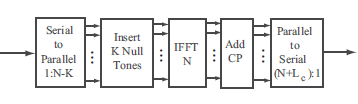
\includegraphics[scale=0.6]{img/OFDDM_modulator.png}
     \caption{Block diagram of the OFDM modulator}
     \label{fig2}
    \end{minipage}\hfill
    \begin{minipage}[b]{0.48\linewidth}  
    \centering  
    \begin{itemize}
    \item[$\bullet$] N : number of subcarriers
    \item[$\bullet$] K : number of null subcarriers
    \item[$\bullet$] $L_c$ : cyclic prefix (against ISI)
    \item[$\bullet$] Block-based modulation technique
    \end{itemize}
        
    \end{minipage}
\end{figure}
\begin{equation}
w[n]=\frac{1}{N} \sum_{m=0}^{N-1} s[m]\exp^{j2\pi\frac{m(n-L_c)}{N}}~for~n=0,...,N+L_c-1
\end{equation}
\end{frame}

\begin{frame}
\frametitle{Demodulation}

\textbf{OFDM} : Devides a frequency-selective channel into N AWGN channels

\begin{figure}[!ht]
         \centering 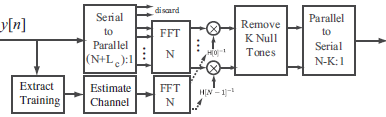
\includegraphics[scale=0.75]{img/OFDDM_demodulator.png}
 \caption{Block diagram of the OFDM demodulator}\label{fig3}  
\end{figure}
\begin{equation}  
 y[n]=\sum_{l=0}^{L} h[l]w[n-l]+v[n]
 \end{equation}
 

\end{frame}

\subsection{Experiment using OFDM}
\subsubsection{Results}

\begin{frame}
\frametitle{Symbol rate}
\begin{center}
	\begin{tabular}{c|c|c}
		  & Narrowband & Wideband\\
		  \hline
	Tx Sample rate & 4 $MSample/s$ & 20 $MSample/s$ \\	  
	Tx Oversample factor & 20 & 4\\
	\textbf{ODFM symbol rate} &  $\textbf{2777.77 symbol/s}$ & $\textbf{69444.44 symbol/s}$ \\ 
	\hline
     & \color{red} \textbf{Flat}  & \color{red} \textbf{Frequency-selective}\\                               
	\end{tabular}
	\label{tab1}
\end{center}


%%$$y[n]=\sum_{l=0}^{L_h} h[l]x[n-l]~where~h[n]=0, \forall n \in (0,1,...,L_h)$$

\begin{itemize}
\item[$\bullet$] Larger symbol rate in wideband than in narrowband.
\item[$\bullet$] Flat-fading : Always the same attenuation on the signal ($L_h=0$)
\item[$\bullet$] Frequency-selective : Different attenuation on the signal ($L_h \neq 0$)
\end{itemize}

\end{frame}

\begin{frame}
\frametitle{Power delay of the channels}

\begin{figure}[!ht]
    \begin{minipage}[b]{0.48\linewidth}
        \centering 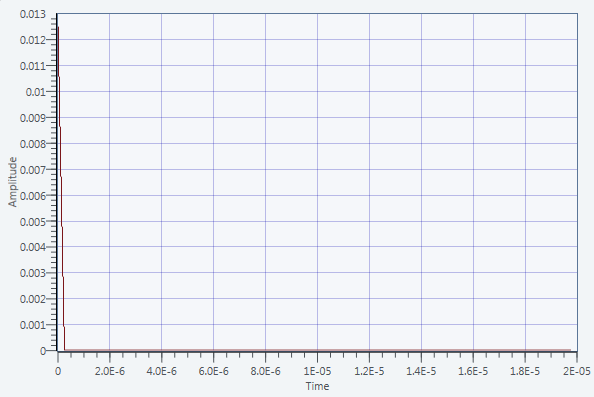
\includegraphics[scale=0.35]{img/power_delay_narrow.png}
     \label{fig4}
    \end{minipage}\hfill
    \begin{minipage}[b]{0.48\linewidth}
         \centering 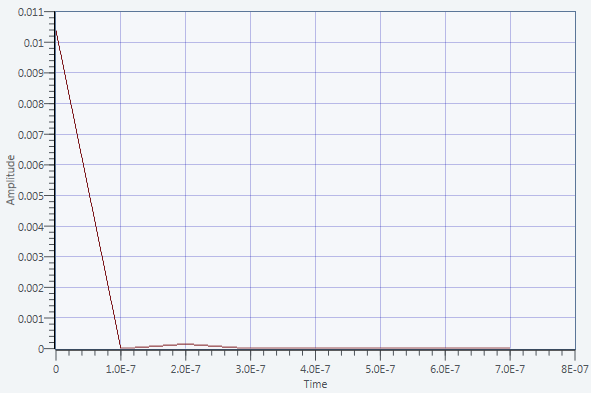
\includegraphics[scale=0.35]{img/power_delay_wideband.png}
    \end{minipage}
\end{figure}
\begin{itemize}
\item[$\bullet$] Narrowband power delay > Wideband power delay  
\end{itemize}
\end{frame}
\subsubsection{Narrowband VS Wideband Channel}
\begin{frame}
\frametitle{Frequency response of each channels}

\begin{figure}[!ht]
    \begin{minipage}[b]{0.48\linewidth}
        \centering 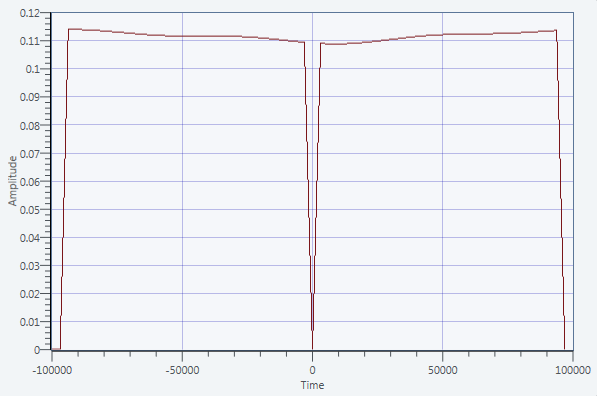
\includegraphics[scale=0.33]{img/channel_response_narrow.png}
     \label{fig2}
    \end{minipage}\hfill
    \begin{minipage}[b]{0.48\linewidth}
         \centering 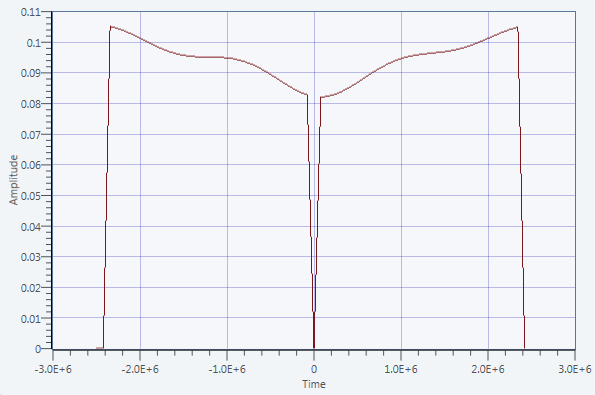
\includegraphics[scale=0.33]{img/channel_response_wideband.png}
    \end{minipage}
\end{figure}
\begin{itemize}
\item[$\bullet$] Flat response in narrowband
\item[$\bullet$] Frequency-selective response in wideband 
\item[$\bullet$] No DC component due to RF distorsion
\end{itemize}

\end{frame}
\subsection{Frequency selectivity of wireless channel}
\begin{frame}
\frametitle{Frequency-selectivity of the channel}

\begin{figure}[!ht]
    \begin{minipage}[b]{0.48\linewidth}
        \centering 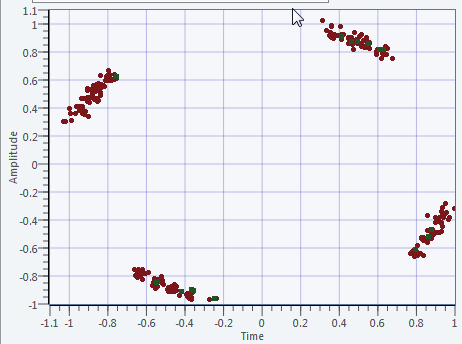
\includegraphics[scale=0.41]{img/multicarrier_200hz.png}
     \label{fig6}
    \end{minipage}\hfill
    \begin{minipage}[b]{0.48\linewidth}
         \centering 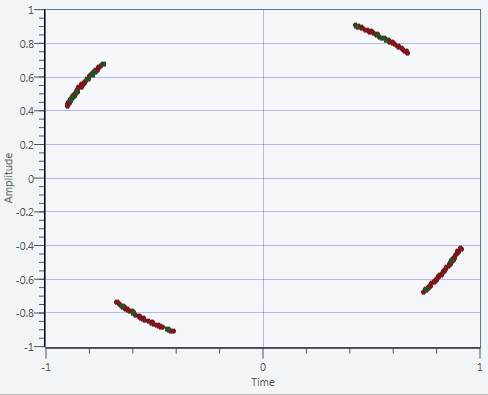
\includegraphics[scale=0.35]{img/SingleCarrier_Offset_200}
\label{fig7}
    \end{minipage}
\end{figure}

\begin{itemize}
\item[$\bullet$] In OFDM, different attenuations on each symbols due to mulipath(Frequency-selective channel)
\end{itemize}
\end{frame}

\begin{frame}
\frametitle{N=64 VS N=1024}
The subcarrier spacing is defined like
\begin{equation}
\Delta_c=\frac{1}{NT} 
\end{equation}
with T the sample period and N the FFT size

\begin{center}
	\begin{tabular}{c|c|c}
		  & $N=64$ & $N=1024$\\
		  \hline
	$\Delta_c$ & $\textbf{15625~kHz}$ & $\textbf{976.56 kHz}$ \\
	\end{tabular}
	\label{tab3}
\end{center}

\begin{itemize}

\item[$\bullet$] Less subcarrier spacing for larger N
\item[$\bullet$] Effect : ICI (inter-carrier interference)
\end{itemize}

\end{frame}

\section{Multi-carrier VS Single-carrier modulation}

\subsection{Major point}
\begin{frame}
\frametitle{Multi VS Single carrier}
\begin{minipage}[t]{0.48\linewidth}
OFDM
\begin{itemize}
\item[$\bullet$] {\color{red} ICI}
\item[$\bullet$] {\color{red} Frequency offset}
\item[$\bullet$] For frequency-selective channel (due to multipath)
\item[$\bullet$] Need more power
\item[$\bullet$] Flexibility: $L_c$, 1/T, N


\end{itemize}
\end{minipage}\hfill
\begin{minipage}[t]{0.48\linewidth}
Single-carrier
\begin{itemize}
\item[$\bullet$] {\color{red} ISI}
\item[$\bullet$] {\color{red} Delay} 
\item[$\bullet$] For flat channel (for little symbol rate)
\item[$\bullet$] Need less power (less bandwidth) 

\end{itemize}

\end{minipage}

\end{frame}

\subsection{Flexibility of OFDM}

\begin{frame}
\frametitle{Influence of 3 parameters on OFDM modulation}

\begin{enumerate}
\item Increasing the number of subcarriers

	\begin{itemize}
		\item[$\bullet$] Make the channel less frequency-selective
		\item[$\bullet$] More sensitive to frequency offset (bad BER)	
	\end{itemize}
	
\item Increasing the bandwidth
	\begin{itemize}
		\item[$\bullet$] Make the channel more frequency-selective
		\item[$\bullet$] Less sensitive to frequency offset
	\end{itemize}

\item The length of the cyclic path	
	\begin{itemize}
		\item[$\bullet$] Avoid ISI
		\item[$\bullet$] Must be greater then $L_h$
	\end{itemize}	

\end{enumerate}

\end{frame}

\end{document}
